\documentclass{beamer}

% Top-aligning columns within a top-aligned frame
% https://tex.stackexchange.com/questions/16447/beamer-top-aligning-columns-within-a-top-aligned-frame
\makeatletter
\newenvironment{myitemize}{%
   \setlength{\topsep}{0pt}
   \setlength{\partopsep}{0pt}
   \renewcommand*{\@listi}{\leftmargin\leftmargini \parsep\z@ \topsep\z@ \itemsep\z@}
   \let\@listI\@listi
   \itemize
}{\enditemize}
\makeatother  

\usepackage[USenglish]{babel}
\usepackage[utf8]{inputenc}
\usepackage{amssymb, amsmath}
\usepackage{bm}
\usepackage{color}
\usepackage{tikz}
\usepackage{url}

\definecolor{links}{HTML}{2A1B81}
\hypersetup{colorlinks,linkcolor=,urlcolor=links}

\usetheme{Boadilla}

\bibliographystyle{apalike}
% make bibliography entries smaller
%\renewcommand\bibfont{\scriptsize}
% Now get rid of all the colours
\setbeamercolor*{bibliography entry title}{fg=black}
\setbeamercolor*{bibliography entry author}{fg=black}
\setbeamercolor*{bibliography entry location}{fg=black}
\setbeamercolor*{bibliography entry note}{fg=black}

\newcommand{\lnorm}[1]{\left\lVert#1\right\rVert^2}
\newcommand{\norm}[1]{\left\lVert#1\right\rVert}

% and kill the abominable icon
\setbeamertemplate{bibliography item}{}

\begin{document}
\title[VITON]{VITON: An Image-based Virtual Try-on Network}  
\author{Radek Bartyzal}
\date{20. 7. 2020} 
\institute{GLAMI AI}

\frame{\titlepage} 
%--------- END Frame 12 -------------
\begin{frame}{Virtual Try On}
Companies:
\begin{itemize}
\item TriMirror, Fits Me
\end{itemize}

\vfill

The key enabling factor behind them is the use of 3D measurements of body shape:
\begin{itemize}
\item captured directly by depth cameras
\item inferred from a 2D image
\end{itemize}

\vfill

Relevant work:
\begin{itemize}
\item infer 3D clothing model from 1 image \cite{cit:3d}
\item a lot of other methods that fail to produce realistic images
\end{itemize}

\end{frame}
%--------- END Frame 12 -------------
\begin{frame}{Example of TriMirror}

\begin{figure}[h]
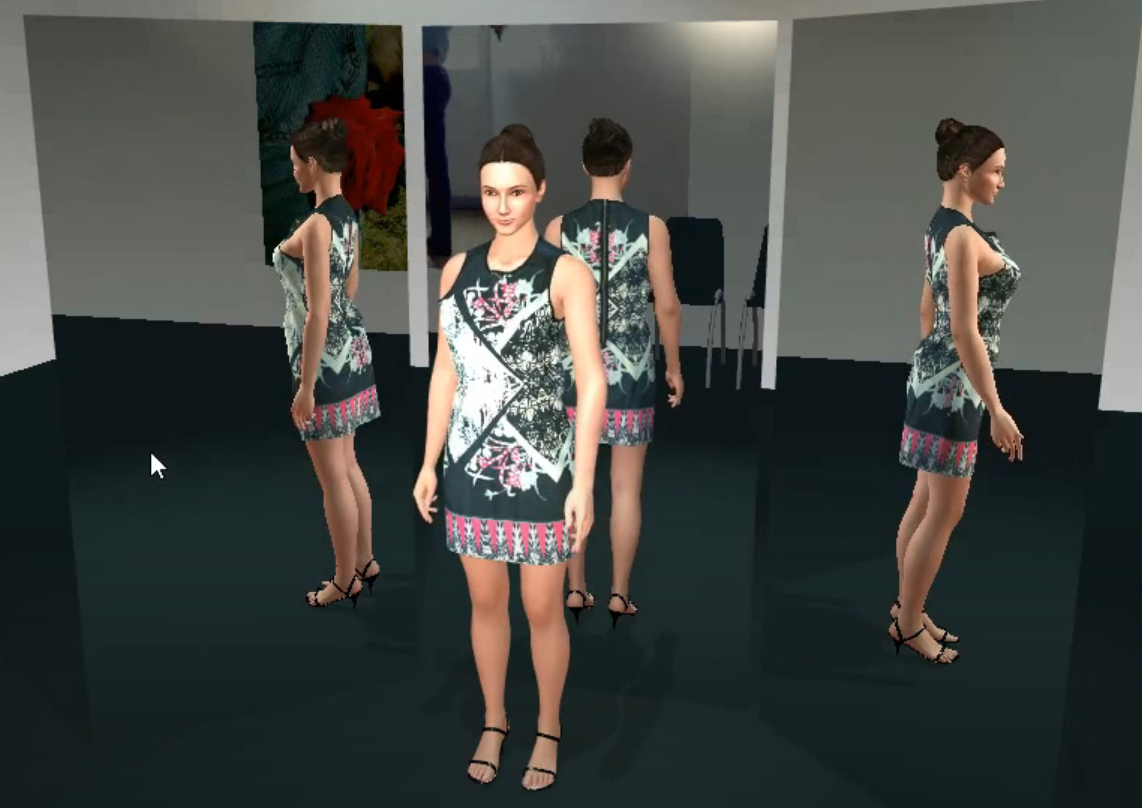
\includegraphics[width=0.9\textwidth]{img/trimirror}
%\caption{TriMirror \cite{cit:trimirror}}
\end{figure}

\end{frame}
%--------- END Frame 12 -------------
\begin{frame}{Motivation}

Idea:
\begin{itemize}
\item do not model the 3D objects, keep it all 2D
\item keep the person's face + body parts = make it personal
\item produce photo-realistic images = no simple avatars
\end{itemize}


\vfill

Input: 
\begin{itemize}
\item 1 (good quality) photo of a person in any clothing
\item 1 product image of a piece of clothing (white background)
\end{itemize}

\vfill

Output:
\begin{itemize}
\item 1 image = original photo with product image put on
\end{itemize}
\end{frame}

%--------- END Frame 12 -------------
\begin{frame}{Example (cherry picked)}

\begin{figure}[h]
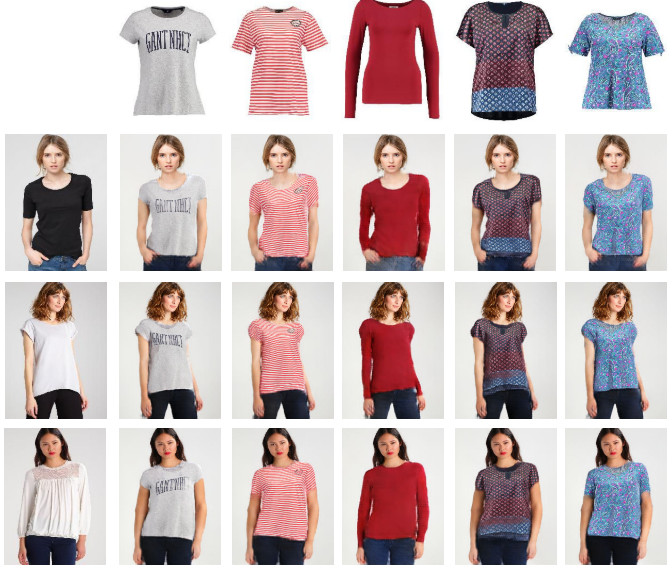
\includegraphics[width=0.9\textwidth]{img/examples}
\end{figure}

\end{frame}
%--------- END Frame 12 -------------
\begin{frame}{Training}

Inputs:
\begin{itemize}
\item reference image $I$ with a person wearing $c$ 
\item product image $c$
\end{itemize}

\vfill

Steps:
\begin{enumerate}
\item create clothing-agnostic representation ($P$) of person in $I$
\item synthesize the reference image $I$ with an encoder-decoder = input is $P$ and $c$, output is attempted reconstruction of $I$ ($I'$) + cloth mask ($M$)
\item use cloth mask $M$ and product image $c$ to generate warped product image $c'$
\item refinement net: input = $c'$, $I'$, output = 1-channel mask $\alpha$
\item result = $\alpha \cdot c' + \alpha \cdot I'$
\end{enumerate}

\end{frame}
%--------- END Frame 12 -------------
\begin{frame}{Clothing-agnostic person representation}

\begin{figure}[h]
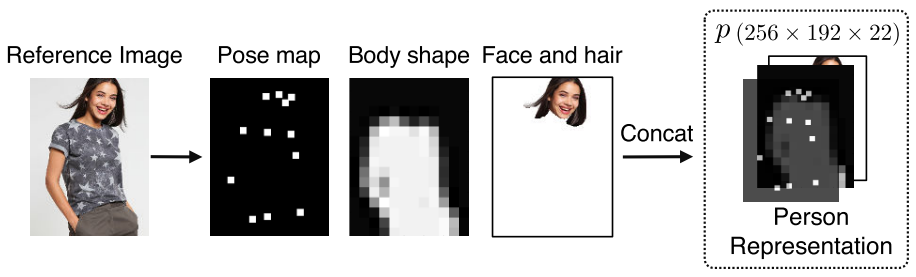
\includegraphics[width=\textwidth]{img/pr}
\caption{Given a reference image I, we extract the pose, body shape and face and hair regions of the person, and use this information as part of input to our generator.}
\end{figure}

\begin{itemize}
\item Pose: SOTA pose estimator
\item Body: downsampled mask (1=human, 0=not) SOTA human parser
\item Face: extract face+hair from human parser
\end{itemize}

\end{frame}
%--------- END Frame 12 -------------
\begin{frame}{Generate coarse image + clothing mask}

\begin{figure}[h]
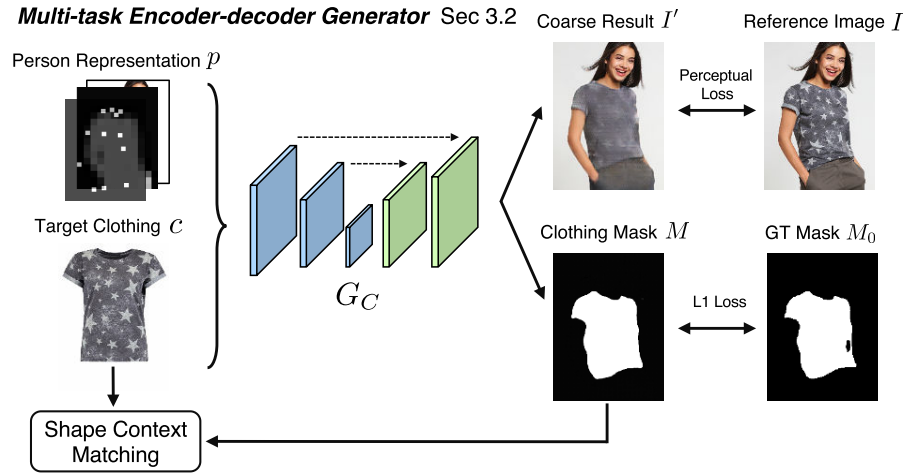
\includegraphics[width=0.9\textwidth]{img/ae}
\caption{$G_C$ = CNN U-Net with skip connections.}
\end{figure}

\end{frame}
%--------- END Frame 12 -------------
\begin{frame}{Generate warped product image}

\begin{figure}[h]
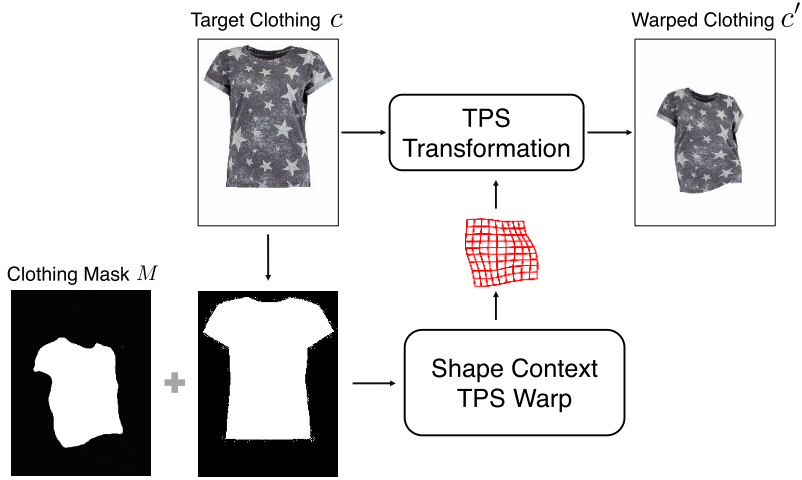
\includegraphics[width=0.7\textwidth]{img/warp}
\caption{Warp the clothing item by estimating a thin plate spline (TPS) transformation with shape context matching.}
\end{figure}

\end{frame}
%--------- END Frame 12 -------------
\begin{frame}{Refinement network}

\begin{figure}[h]
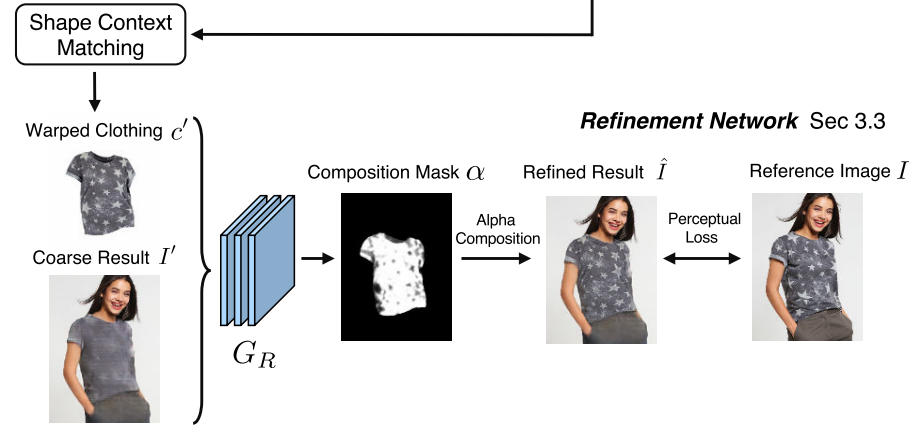
\includegraphics[width=\textwidth]{img/refine}
\caption{Simple CNN.}
\end{figure}

\end{frame}
%--------- END Frame 12 -------------
\begin{frame}{Effect of removal of body and pose}

\begin{figure}[h]
\includegraphics[width=\textwidth]{img/remove}
\caption{For each method, we show its coarse result and predicted clothing mask output by the cor- responding encoder-decoder generator.}
\end{figure}

\end{frame}
%--------- END Frame 12 -------------
\begin{frame}{Failure cases}

\begin{figure}[h]
\includegraphics[width=\textwidth]{img/fails}
\caption{Failure cases of our method due to rarely-seen poses (example on the left) or a huge mismatch in the current and target clothing shapes (right arm in the right example).}
\end{figure}

\end{frame}
%--------- END Frame 12 -------------
\begin{frame}{Results on real photos from COCO dataset}

\begin{figure}[h]
\includegraphics[width=0.8\textwidth]{img/wild}

\end{figure}

\end{frame}
%--------- END Frame 12 -------------
\begin{frame}{Conclusion}

What is required:
\begin{itemize}
\item trained pose estimator
\item trained human parser = pixel-wise image segmentation of body parts
\end{itemize}

\vfill

New version O-VITON:
\begin{itemize}
\item similar principle
\item requires training:
\begin{itemize}
\item pixel-wise semantic segmentation of body parts + clothing
\item DensePose network which captures the pose and body shape
\end{itemize}
\end{itemize}

\end{frame}

%--------- END Frame 12 -------------
\begin{frame}{Sources}
\begin{thebibliography}{0}

  \bibitem[1]{cit:paper} 1. Han, Xintong, et al. "Viton: An image-based virtual try-on network." Proceedings of the IEEE conference on computer vision and pattern recognition. 2018. \url{https://arxiv.org/abs/1711.08447} 
  \bibitem[2]{cit:trimirror} 2. TriMirror video \url{https://www.youtube.com/watch?v=vYJ19Z9i-zY} 
  
  \bibitem[3]{cit:3d} 3. S. Yang, T. Ambert, Z. Pan, K. Wang, L. Yu, T. Berg, and M. C. Lin. Detailed garment recovery from a single-view image. In ICCV, 2017
\end{thebibliography}

\end{frame}

 
\end{document}
